\chapter{Technique Overview}\label{ch:research}
The objective is to create an overview of techniques in the field which may be used to solve the
problem detailed in Chapter~\ref{ch:problem}.
According to the methodology detailed in~\ref{se:methodology}, first a taxonomy is introduced
which facilitates the analysis and comparison of techniques.
The subsequent search for literature which lays the foundation for an overview over current research
is documented.
Lastly, the advances in the field are placed in the correct position and analyzed.

\section{Taxonomy of Pipeline Steps}
Before getting into current research level, a base of knowledge about the field has to be layed.
A taxonomy is created for this which is useful to classify and give context to innovations in the
field.
The partition of tasks and categorization of approaches is conducted according to overview literature
such as~\cite{long_scene_2021,chen_text_2021,cong_comparative_2019} and related work sections of
research in the field such
as~\cite{qiao_text_2021,sheng_centripetaltext_2021,liu_accurate_2020,deng_pixellink_2018}.
To create the overview the necessary steps in the process of \ac{STS} needs to be highlighted,
from preprocessing to classifying the identified
text~\citep{long_scene_2021, sourvanos_challenges_2018}.
The ways in which the respective issues for the steps are solved are identified from literature,
listed and explained alongside.
\begin{figure}[h]
    \centering
    \resizebox{\linewidth}{!}{
\begin{tikzpicture}[
    every node/.style={draw=black,thin,anchor=west, minimum height=2.5em},
    lroot/.style={%
        edge from parent fork down,
        level distance=0.5cm,
        text centered, text width=3cm},
    lone/.style={%
        text centered, text width=3cm,
        level distance=0.5cm},
    ltwo/.style={%
        text centered, text width=3cm,
        level distance=0.5cm},
    lthree/.style={%
        rounded corners,
        grow=down, xshift=-0.8cm,
        text centered, text width=3cm,
        edge from parent path={(\tikzparentnode.205) |- (\tikzchildnode.west)}},
    level1/.style ={level distance=1.2cm},
    level2/.style ={level distance=2.4cm},
    level3/.style ={level distance=3.6cm},
    level4/.style ={level distance=4.8cm},
    level5/.style ={level distance=6.0cm},
    level 1/.style={sibling distance=8cm},
    level 1/.append style={level distance=1.5cm},
    level 2/.style={sibling distance=4cm},
    level 2/.append style={level distance=1.5cm},
]
%   \draw[help lines] (0,0) grid (4,3);

    % lroot
    \node[anchor=south,lroot]{STS}
    [edge from parent fork down]
        child{node [lone] {STD}
            child{node [ltwo] {Regressor \\ based}
                child[lthree,level1] {node {Feature \\ Extraction}}
                child[lthree,level2] {node {BB \\ Regresseion}}
                child[lthree,level3] {node {IOU \\ matching}}
            }
            child{node [ltwo] {Segmentation \\ based}
                child[lthree,level1] {node {Sub-components \\ segmentation}}
                child[lthree,level2] {node {Text \\ reconstruction}}
            }
        }
        %
        child{node [lone] {STR}
            child{node [ltwo] {Regressor \\ based}
                child[lthree,level1] {node {Image \\ preprocessing}}
                child[lthree,level2] {node {Character \\ segmentation}}
                child[lthree,level3] {node {Character \\ recognition}}
            }
            child{node [ltwo] {Segmentation \\ based}
                child[lthree,level1] {node {Image \\ preprocessing}}
                child[lthree,level2] {node {Feature \\ extraction}}
                child[lthree,level3] {node {Sequence \\ modelling}}
                child[lthree,level4] {node {Prediction}}
            }
        }
        %
        child{node [lone] {E2E}
            child{node [ltwo] {Two Stage}
                child[lthree,level1] {node {STD}}
                child[lthree,level2] {node {STR with \\ feature maps}}
            }
            child{node [ltwo] {One Stage}
                child[lthree,level1] {node {STD \& STR \\ Parallel}}
            }
        };

\end{tikzpicture}
}%


\begin{comment}
\begin{tikzpicture}[
    font=\scriptsize,
    edge from parent fork down,
    level distance=1.75cm,
    every node/.style={
            rectangle,
            minimum height=6mm,
            align=center,
            text depth = 0pt,
    },
    edge from parent/.style={draw=black},
    category/.style={Rectangle},
    step/.style={Circle}
]
    \Tree [.STS
        [.{STD}
            [.{Feature \\ Extraction} ]
            [.{BB Regression} ]
        ]
        [.{STR}
            [.{Preprocessing} ]
            [.{Feature \\ Extraction} ]
            [.{Sequence \\ Modelling} ]
            [.{Prediction} ]
        ]
    ]
\end{tikzpicture}
\end{comment}

\caption{Pipeline taxonomy and respective steps\label{fig:pipelineSteps}}
\end{figure}
Figure~\ref{fig:pipelineSteps} shows tasks and their respective approaches which are associated
with \ac{STS}.
\ac{STD} and \ac{STR} only incorporate a part of \ac{STS}, while E2E
incorporate both \ac{STD} and \ac{STR} techniques to solve \ac{STS}~\citep{long_scene_2021}.
Therefore this section will first discuss the two parts, to then later combine them.

For \ac{STD} two main categories of approaches can be identified: segmentation based and \ac{BB}
regression based~\citep{long_scene_2021,sheng_centripetaltext_2021,liu_accurate_2020}.
The regression based category draws heavy inspiration from the field of object
detection~\citep{long_scene_2021,liu_accurate_2020}.
This is only natural as text detection can be seen as a type of object
detection~\citep{liu_accurate_2020,long_scene_2021}.
For object detection inspired \ac{STD} there are two methods: one stage and two
stage~\citep{long_scene_2021}.
Both localize text instances as a whole (in the form of a
\ac{BB})~\citep{long_scene_2021,sheng_centripetaltext_2021}.
One stage approaches are modelled after~\cite{liu_ssd_2016}, Single Shot MultiBox
Detector (SSD) and~\cite{redmon_you_2016}, You Only Look Once (YOLO).
They have in comon that \acp{BB} are regressed once and not changed or optimized
afterwards~\citep{redmon_you_2016,liu_ssd_2016}, as opposed to the \ac{ROI} based approach with two
stages~\citep{girshick_rich_2014}.
\begin{figure}[ht]
    \centering
    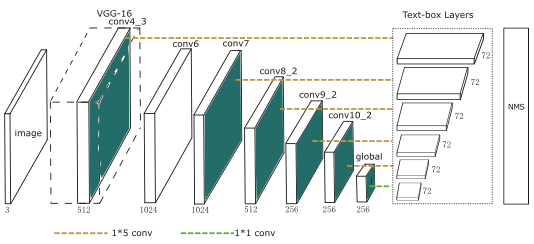
\includegraphics[width=0.8\textwidth]{img/STD-seg-free-Liao-TextBoxes-2017.png}
    \caption[One stage, BB regression based STD architecture]{%
        Example for a one stage, BB regression based STD
        architecture~\citep{liao_textboxes_2017}\label{fig:STD-segfree-ssd}
    }
\end{figure}
The basic approach is explained with the example of~\cite{liao_textboxes_2017} (see
Figure~\ref{fig:STD-segfree-ssd}) which is based on SSD.\
Note that the approach is modeled to recognize horizontal text instances~\citep{liao_textboxes_2017}.
It uses 13 layer convolutional network inspired by the VGG architecture (blocks of: two or
three $3\times3$ conv layers followed by a $2\times2$ max pooling layer with stride 2) for feature
extraction~\citep{liao_textboxes_2017,simonyan_very_2015}.
Note that the spatial padding added for convolution ensures that spatial dimensions are
preserved~\citep{simonyan_very_2015}.
Afterwards come nine additional layers which continuously downsample, the output of six of them
is separately used as feature maps for \ac{BB} regression~\citep{liao_textboxes_2017}.
The downsampling and \ac{BB} regression for different layers helps detect text instances of different
scales~\citep{liu_ssd_2016}.
Each spatial location on the feature map can be traced back to a region on the input
image~\citep{long_scene_2021}.
The \ac{BB} regression is carried out by six text-box layers which predict how certain ($c_1,c_2$)
the prediction is a text instance or background and where the text instance is ($x,y,w,h$).
Note that the output is not the location of a \ac{BB} but the offset to the
respective anchor box~\citep{liao_textboxes_2017,long_scene_2021}.
Anchor boxes are predefined to give bias towards sizes and aspect ratios of
text~\citep{liao_textboxes_2017}.
The text-box layers are the difference to the SSD approach for normal object
detection~\citep{liao_textboxes_2017,liu_ssd_2016}.
These layers use $1\times5$ filters to adjust to larger aspect ratios~\citep{liao_textboxes_2017}.
Each text-box layer has 72 filters (12 anchor boxes $\cdot$ 6 values per prediction), the filters
are slided accross the input features generating 12 predicted \ac{BB} per
position~\citep{liao_textboxes_2017}.
The \acp{BB} of all layers are then subjected to the process of \ac{NMS} to filter out the best
\ac{BB} for each possible text instance~\citep{liao_textboxes_2017}.
For this \ac{NMS} is used: of all detections which overlap more than a threshhold $\phi$ only the
with the highest confidence score ($c$) is kept~\citep{hosang_learning_2017}.

The R-CNN which builds the foundation for \ac{ROI} based text detection, was introduced
by~\cite{girshick_rich_2014} and improved by~\cite{girshick_fast_2015} (Fast
R-CNN),~\cite{ren_faster_2015} (Faster R-CNN) and~\cite{he_mask_2018} (Mask R-CNN).
Note that 2-stage methods are fully differentiable and thus end to end trainable since
Faster R-CNN (like 1-stage methods)~\citep{ren_faster_2015,long_scene_2021}.
The two stages consist of: \acp{ROI} regression, \acp{BB}
adjustments~\citep{jiang_r2cnn_2017, ren_faster_2015}.
The \ac{STD} approach introduced by~\cite{jiang_r2cnn_2017} (see Figure~\ref{fig:STD-segfree-rcnn})
uses Faster R-CNN.%
Unlike the previous approach, the architecture is designed to detect multioriented text instances
as such~\citep{jiang_r2cnn_2017,liao_textboxes_2017}.
\begin{figure}[ht]
    \centering
    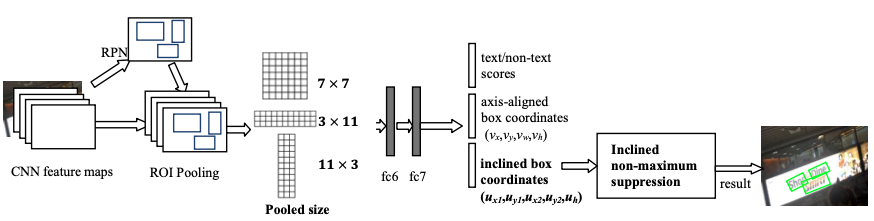
\includegraphics[width=0.8\textwidth]{img/STD-seg-free-Jiang-R2CNN-2017.png}
    \caption[Two stage, BB regression based STD architecture]{%
        Example for a two stage, BB regression based STD
        architecture~\citep{jiang_r2cnn_2017}\label{fig:STD-segfree-rcnn}
    }
\end{figure}
Like with the one stage approach, the two stage approach starts with feature extraction from the
image with a convolutional layers~\citep{jiang_r2cnn_2017}.
Feature extraction can be performed with the VGG architecture~\citep{jiang_r2cnn_2017}, like in
the previous approach.
The generated feature map is used by a \ac{RPN}.
Like with the previously explained approach, the feature maps are used to regress the offset
respective to bounding boxes.
The bounding boxes are still axis aligned at this point~\citep{jiang_r2cnn_2017}.
In contrast to the previous SSD based approach, only one feature map is used in conjunction with
\ac{BB} regression~\citep{jiang_r2cnn_2017}.
The \ac{RPN} from Faster R-CNN is adjusted to use smaller scale anchor boxes to adapt to
text~\citep{jiang_r2cnn_2017}.
Note that R-CNN and Fast-RCNN used the slower Sequential Search algorithm instead of an
\ac{RPN}~\citep{girshick_rich_2014,girshick_fast_2015}.
The resulting \acp{BB} are called \acp{ROI}~\citep{ren_faster_2015,jiang_r2cnn_2017}.
They are used for \ac{ROI} pooling in conjunction with the original feature maps.
This layer uses max pooling to convert the spatial features corresponding to the location of the
\ac{ROI} to a small feature map~\citep{girshick_fast_2015}.
In the case of this example, \ac{ROI} pooling is used to create three feature maps with different
aspect ratios ($7\times7, 3\times11, 11\times3$) which are concatenated for the next
step~\citep{jiang_r2cnn_2017}.
The second stage is to predict a confidence score (text, background) for each \ac{ROI} and to
refine them by regressing values ($x_1,y_1,x_2,y_2,h$) that allow for inclined boxes to account for
rotated text~\citep{jiang_r2cnn_2017}.
At last the resulting \acp{BB} are filtered by inclined \ac{NMS} which is adjusted to the
incline \ac{BB}~\citep{jiang_r2cnn_2017}.

The basis for the segmentation based methods is the fact that every part of the text instance can
be used to verify that there is text~\citep{long_scene_2021}.
Because of this, sub-text components can be detected separately and then used to re-construct a text
instance~\citep{long_scene_2021}.
Segmentation based methods can roughly be summed up in two categories: pixel based and component
based~\citep{long_scene_2021}.
Like with \ac{BB} regression based methods, example architectures are explained in order to
describe their categories more clearly.
The paper~\cite{deng_pixellink_2018} introduced a pixel based \ac{STD} approach.
\begin{figure}[ht]
    \centering
    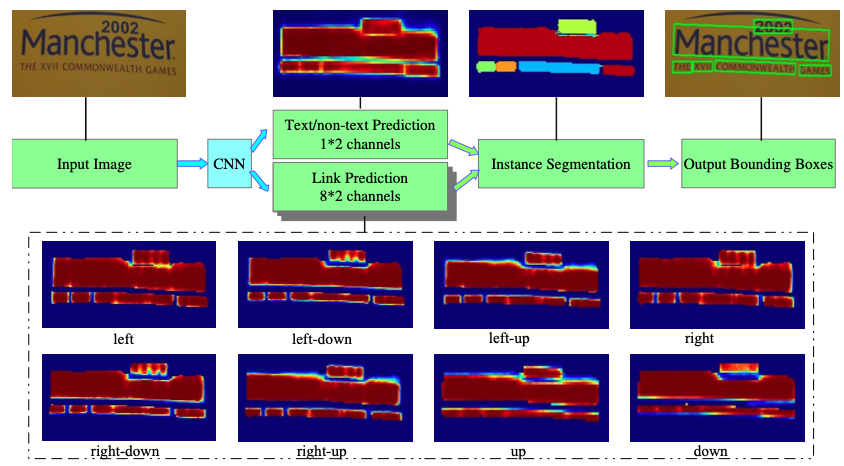
\includegraphics[width=0.7\textwidth]{img/STD-seg-based-architecture-Deng-PixelLink-2018.png}
    \caption[Pixel, segmentation based STD architecture]{%
        Example for a pixel, segmentation based STD
        architecture~\citep{deng_pixellink_2018}\label{fig:STD-segbased-pixel-architecture}
    }
\end{figure}
Figure~\ref{fig:STD-segbased-pixel-architecture} shows the approch's architecture.
Figure~\ref{fig:STD-segbased-pixel-CNN} shows the \ac{CNN} structure for feature extraction
(until conv5) which is basically VGG architecture with the fully connected layers exchanged with
another convolutional stage~\citep{deng_pixellink_2018}.
The feature extraction followed by two heads which either predict text/non-text or
links~\citep{deng_pixellink_2018}.
The structure which combines downsampled feature maps with later upsampled ones is inspired
by~\cite{long_fully_2015}.
Continuous downsampling and and combining those layers with later, upsampled layers helps
to combine coarse, higher level information with fine, lower level
information~\citep{long_fully_2015}.
The upsampling is performed with bilinear interpolation~\citep{deng_pixellink_2018}.
Depending on which head is used, the $1\times1$ convolution layers either have 2 or $2\cdot8$ filters.
Counted together, the model has 18 output channels~\citep{deng_pixellink_2018}.
The $1\times1$ convolution layers are also used for upsampling (deconvolution,
see~\cite{noh_learning_2015,long_fully_2015} for an in depth explanation)~\citep{deng_pixellink_2018}.
The 2 filters are used to predict text/non-text for each pixel, while the other 16 filters predict
the links~\citep{deng_pixellink_2018}.
The text/non-text head essentially performs semantic segmentation, that is to categorize each
pixel to its type~\citep{deng_pixellink_2018}.
For every neighbor there is a negative and a positive score.
A pixel has eight neighbors: left, left-down, left-up, right, right-down, right-up, up, down.
Each of the $2\cdot8$ filters is responsiblde for link a neighbor~\citep{deng_pixellink_2018}.
\begin{figure}[ht]
    \centering
    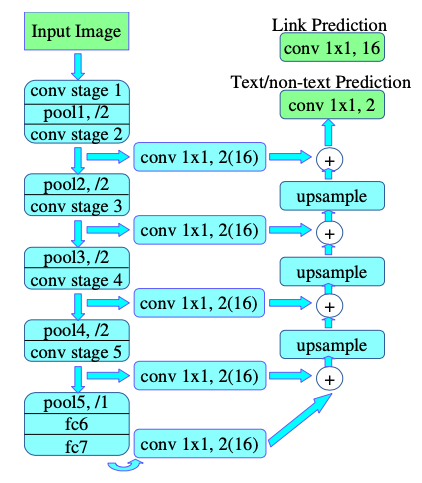
\includegraphics[width=1\textwidth]{img/STD-seg-based-CNN-Deng-PixelLink-2018.pdf}
    \caption[Feature extractor and prediction head for pixel segmentation]{%
        PixelNet CNN feature extractor with head structure for pixel
        segmentation\label{fig:STD-segbased-pixel-CNN}
    }
\end{figure}
After both links and text/non-text pixels have been predicted, they are combined for instance
segmentation~\citep{deng_pixellink_2018}.
The link layers are used to indicate whether two text pixels are grouped together an thus belong to
the same instance~\citep{deng_pixellink_2018}.
The output is a dense prediction map with the same spatial structure as the input
image~\citep{deng_pixellink_2018}.
A bounding box can then be extracted by laying minimum area rectangles over the
instances~\citep{deng_pixellink_2018}.

The second segmentation based category for \ac{STD} segments components which are local regions of
text that can overlap one or more characters~\citep{long_scene_2021}.
\begin{figure}[ht]
    \centering
    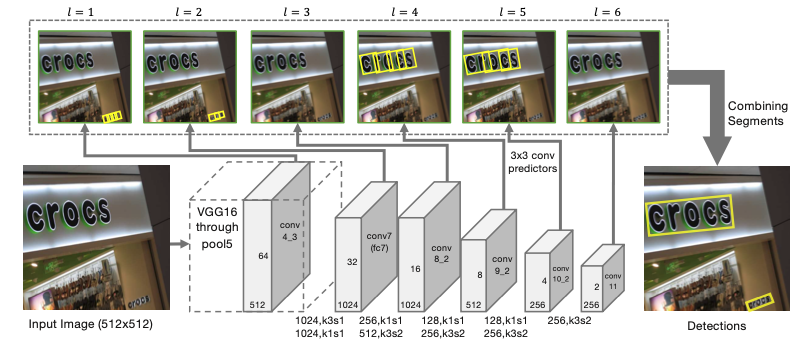
\includegraphics[width=0.9\textwidth]{img/STD-seg-based-architecture-Shi-Detecting-2017.png}
    \caption[Sub-component, segmentation based STD architecture]{%
        Example for a sub-component, segmentation based STD
        architecture~\citep{shi_detecting_2017}\label{fig:STD-segbased-component-architecture}
    }
\end{figure}
The architecture (see Figure~\ref{fig:STD-segbased-component-architecture})
from~\cite{shi_detecting_2017} is used as an example for this category.
Like the one-stage, \ac{BB} regression based \ac{STD} approach, the feature extraction \ac{CNN} of
this approach is taken from SSD and thus VGG, the difference is reflected in the prediction
layers~\citep{shi_detecting_2017,liu_ssd_2016,simonyan_very_2015}.
Instead of detecting whole \acp{BB}, the networks predicts both subcomponents and links at multiple
scales~\citep{shi_detecting_2017}.
The convolutional prediction is carried out with seven $3\times3$ filters followed by a softmax
nonlinearity for normalization.
The segments are given by the values $x_s,y_s,w_s,h_s,\theta_s$ which offset an anchor box as well
as confidence scores $c_1,c_2$~\citep{shi_detecting_2017}.
Links are used to separate the segments and are accordingly used to separate neraby
words~\citep{shi_detecting_2017}.
The prediction layer applies convolution, like with $c_1,c_2$ for every neighbor and cross layer
neighbor a positive and a negative value is predicted~\citep{shi_detecting_2017}.
\begin{figure}[ht]
    \centering
    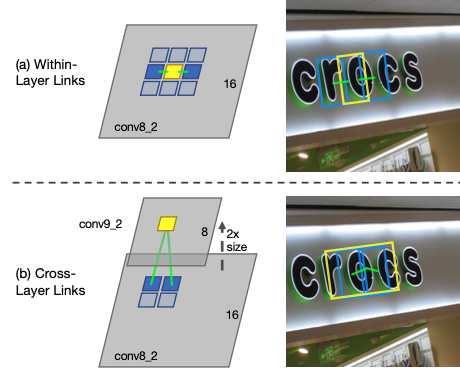
\includegraphics[width=0.5\textwidth]{img/STD-seg-based-links-Shi-Detecting-2017.png}
    \caption[Predicting links for segmentation based STD]{%
        Visualization for prediction of links within and cross layers for segmentation based
        STD~\citep{shi_detecting_2017}\label{fig:STD-segbased-component-links}
    }
\end{figure}
% XXX: are equations really needed?
Within layer links are predicted for the neighbors of a space in the predicted feature map
(see Figure~\ref{fig:STD-segbased-component-links} (a),
Equation~\ref{eq:STD-segbased-subcomp-same-layer})~\citep{shi_detecting_2017}.
\begin{equation}\label{eq:STD-segbased-subcomp-same-layer}
    \mathcal{N}_{s^{x,y,l}}^w =
        \frac{{\{s^{(x',y',l)}\}}_{x-1\leq x'\leq x+1,y-1\leq y'\leq y+1}}{s^{(x,y,l)}}
\end{equation}
The cross layer links on the other hand are predicted by using the 4 cross layer neighors of the
feature map of the preceding predictor~\citep{shi_detecting_2017}.
(see Figure~\ref{fig:STD-segbased-component-links} (b),
Equation~\ref{eq:STD-segbased-subcomp-cross-layer})~\citep{shi_detecting_2017}.
\begin{equation}\label{eq:STD-segbased-subcomp-cross-layer}
    \mathcal{N}_{s^{x,y,l}}^c = {\{s^{(x',y',l-1)}\}}_{2x\leq x'\leq 2x+1,2y\leq y'\leq 2y+1}
\end{equation}
These cross layer links are used to connect segments on different scales~\citep{shi_detecting_2017}.
The network architecture designed so that the preceding feature map is twice the sice (spatial
dimensions) of the current which is necessary to extract the right
locations~\citep{shi_detecting_2017}.
Before reconstruction the text instances, segments are filtered by their confidence
scores~\citep{shi_detecting_2017}.
To reconstruct, the predictions are taken as a graph: segments are nodes, links are edges.
Depth-first search is applied to the graph to find connected components and thus text
instances~\citep{shi_detecting_2017}.

% FIXME: how to begin?
Examples
\begin{itemize}
    \item Segmentation based approach~\cite{liao_scene_2018}
    \item Segmentation less: (important to mention improvements made)
        CTC ---~\cite{shi_end--end_2017},
        Attention ---~\cite{sutskever_sequence_2014}
\end{itemize}

Segmentation less
\begin{itemize}
    \item mention dependency on lexicons
    \item Steps: Preprocessing, Feature Extraction, Sequence Modelling, Prediction
    \item preprocessing, text enhancement: remove distortions, background; improve resolution,
        recover degraded text
        \begin{itemize}
            \item Spatial Transformer Networks (for distortions)
        \end{itemize}
    \item feature extraction: encode image into feature space
        \begin{itemize}
            \item ResNet
                \begin{itemize}
                    \item aggressive downsampling
                    \item $3\times3$ best kernel size
                    \item Gradient saving $\rightarrow$ Res block, Res Bottleneck, Res Grouped
                    \item batch normalization
                    \item 32,50,150,\ldots
                \end{itemize}
            \item GoogLeNet
        \end{itemize}
    \item Sequence and Prediction
        \begin{itemize}
            \item CTC
            \item Encode-Decoder/Attention
            \item Lexicon Free Models!
        \end{itemize}
\end{itemize}

E2E
\begin{itemize}
    \item trainable as one?
    \item Bestandteile nicht zwangsweise sequentiell
    \item two step or two stage pipeline
\end{itemize}

\begin{table}[ht]
    \centering\scriptsize
    \begin{tabular}{p{.05\textwidth}p{.09\textwidth}p{.16\textwidth}p{.55\textwidth}}
        Task & \multicolumn{2}{c}{Approach category} & Identifying properties \\
        \toprule
        STD & Seg free & & Localize whole instances  \\
            & & 1-stage & direct \ac{BB} regression \\
            & & 2-stage & find \acp{ROI}, adjust \acp{ROI} for better fit \\
            & Seg based & & Localize sub text components to reconstruct instance \\
            & & Pixel-level & Pixel level segmentation \\
            & & Component-level & Sub-component level segmentation \\
        \midrule
        STR & Seg based & & Character segmentation and classification\\
            & Seg free & & Text instance recognition \\
            & & CTC based &  \\
            & & Attention based & Encoder-Decoder Mechanism \\
        \midrule
        E2E & 2-step & & \\
            & Parallel & & \\
        \bottomrule
    \end{tabular}
    \caption{Tasks, method categories and identifying propertis\label{tb:steps-properties}}
\end{table}
% FIXME: after all explained: Note that mixtures of the categories are possible in practice,
%           the categorization is applied to help compare approaches (give example for mixture)

\section{Literature Search}\label{se:litSearch}
% FIXME: literature quellen reinbringen
This section documents the search for literature which provides the content for the subsequent
overview of innovation.
For this, important \ac{DL} techniques and notable advances along with their properties are researched
and presented.
For a literature review, it is important to report how the information was found and
synthesized~\citep{torraco_writing_2005}.
The strategy for researching current research is most important for a literature
review~\citep{snyder_literature_2019}.
This includes databases and keywords that were used, as well as exclusion criteria that were
enforced~\citep{torraco_writing_2005}.
The literature is identified through searching in the Google Scholar database.
The search is executed with keywords such as, but not only: Deep Learning, Text Detection,
Text Recognition, Text Spotting, Scene Text, Pipeline.
% XXX: update keywords
A criterion for further examination is an appropriate amount of citations for the piece of literature
in question.
Additionally, literature is selected through citations for and by literature which has already been
identified as important.
All research after 2018 which pertains to extracting scene text is regarded as relevant.
Standard \ac{OCR} solutions may not hold validity in practice, as the image and text conditions can
vary in the defined problem~\citep{chen_text_2021}.
The delimination from Section~\ref{se:problem} of course holds for this chapter and only literature
which concerns advances for the \ac{DL} model architecture will be regarded as important for the
scope of this thesis.
This extends to the whole pipeline from preprocessing an image to the final result of the model.

% FIXME: hierarchical graphic with found papers
% FIXME: describe proceeding


\section{State of the Art Methods}

text enhancement:~\cite{chen_text_2021}
model pruning:~\cite{niu_26ms_2019}
integer inference:~\cite{ignatov_ai_2019}
